\subsubsection{28.12.2015}
\textit{\textbf{Time frame:}} 16:00-22:00 \newline
На сложном роботе за сегодня было сделано
1) поднята наклонная плоскость, т. к. она цепляла пол и нельзя было ехать.
2) изменена программа для езды, регулировка скорости и танковый разворот.
3) тестирование подъёмника, откуда выяснилось, что при определённом выдвижение подъёмника можно полностью заехать на горку, но нужно сделать механизм крепления к балке после заезда. Также был сожжён dc-мотор, т.к. мощности двух моторов не хватает для выдвижение подъёмника
4) тестирование корзины. Механизм выдвижения в бок работает, а также механизмы для открытия корзины и опракидавоние игровых элементов тоже работают.
5) стало понятно, что надо сделать передачу на нижнюю ось схвата иначе оси будут вращаться в разные стороны

\begin{figure}[H]
	\begin{minipage}[h]{0.58\linewidth}
		\center{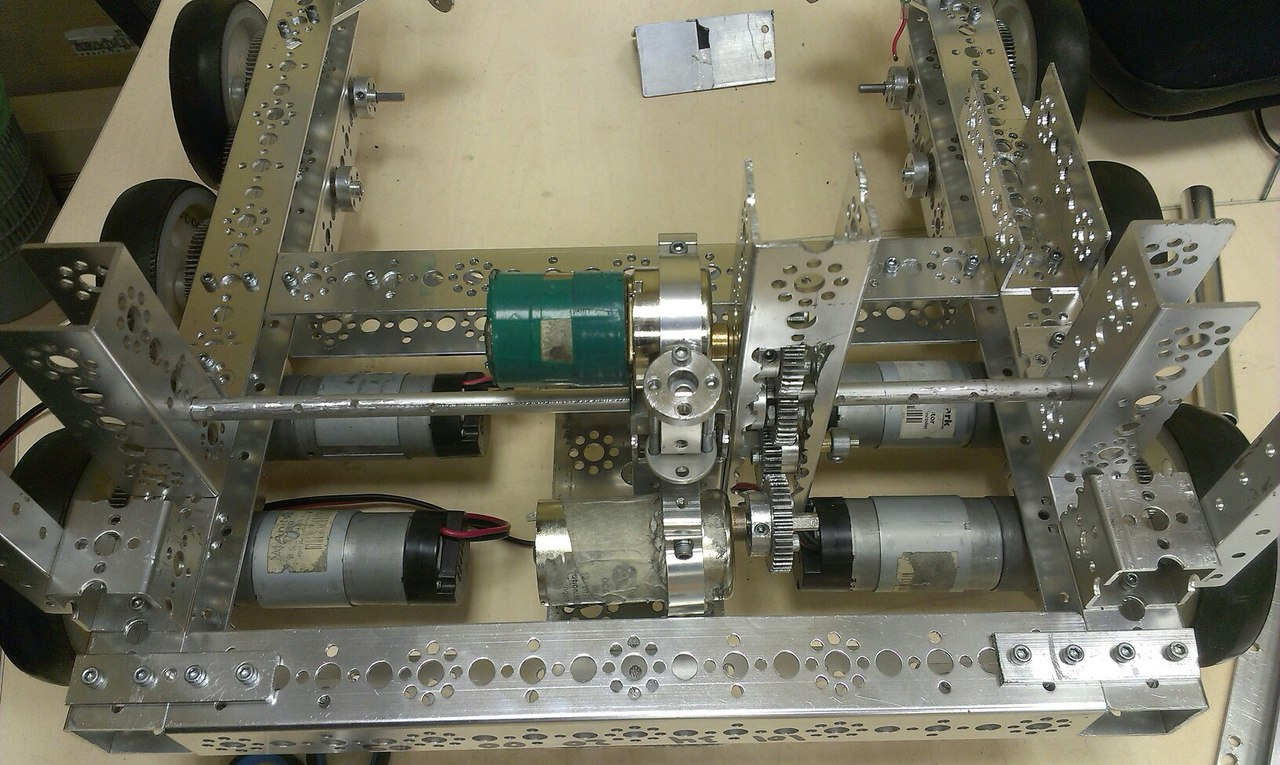
\includegraphics[scale=0.2]{3Engineering/5Team_meetings/days_of_meetings/2015.12.17/images/01}}
		\caption{Winch installed onto the carriage}
	\end{minipage}
	\hfill
	\begin{minipage}[h]{0.37\linewidth}
		\center{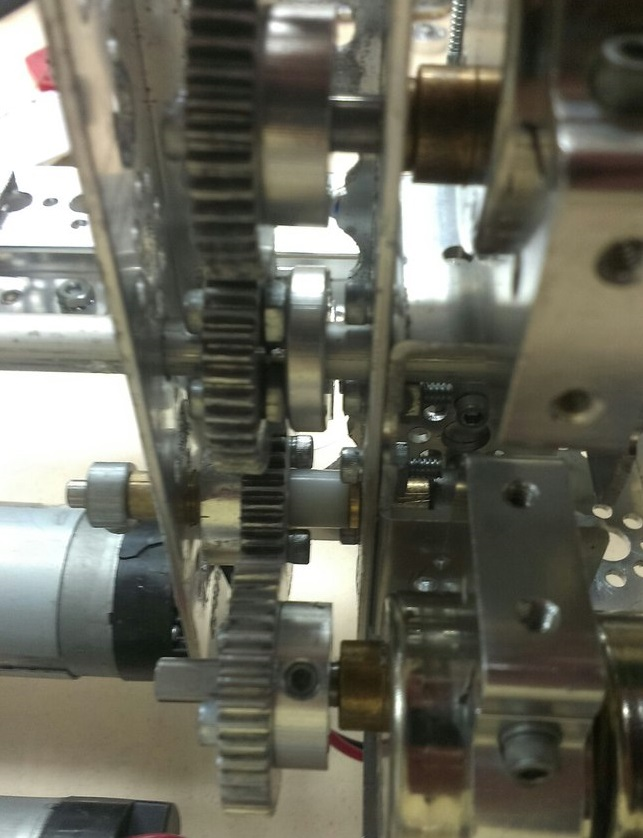
\includegraphics[scale=0.22]{3Engineering/5Team_meetings/days_of_meetings/2015.12.17/images/02}}
		\caption{The construction of the winch}
	\end{minipage}
\end{figure}
